\documentclass[12pt]{article}
\usepackage[a4paper,margin=0.75in]{geometry}
\usepackage[utf8]{inputenc}
\usepackage[OT1]{fontenc}
\usepackage[table,usenames,dvipsnames]{xcolor}
\usepackage{array}
\usepackage{varwidth}
\usepackage{tabularx}
\usepackage{amsmath}
\usepackage{hyperref}
\usepackage{enumitem}
\usepackage{graphicx}
\usepackage{tcolorbox}
\renewcommand*\familydefault{\sfdefault}

\newtcolorbox{mybox}[3][]
{
  colframe = #2!25,
  colback  = #2!10,
  coltitle = #2!20!black,  
  title    = {#3},
  #1,
}

\hypersetup{
    colorlinks=true,
    linkcolor=blue,
    filecolor=magenta,      
    urlcolor=cyan,
    pdftitle={Overleaf Example},
    pdfpagemode=FullScreen,
}

\title{\textbf{COL774 Assignment 2}}
\author{Aniruddha Deb \\ \texttt{2020CS10869}}
\date{October 2022}

\begin{document}

\maketitle

\section{Naive Bayes}

\begin{enumerate}[label=(\alph*)]
  
    \item Naive Bayes was implemented using the \textbf{Multinomial Event Model} as discussed in class, which uses the frequency of the words rather than just their presence. The vocabulary was learnt from the training dataset, and any words not in the vocabulary in the test dataset were ignored. With this implementation, the following results were obtained:
    \begin{enumerate}
        \item An accuracy of $79.313\%$ on the test dataset, with 7501/10000 positive examples and 4396/5000 negative examples correctly classified
        \item The following word clouds were obtained. Note that there are a lot of stopwords, which we remove in part (d)
    \end{enumerate}
    \begin{center}
        \begin{tabular}{c c}
            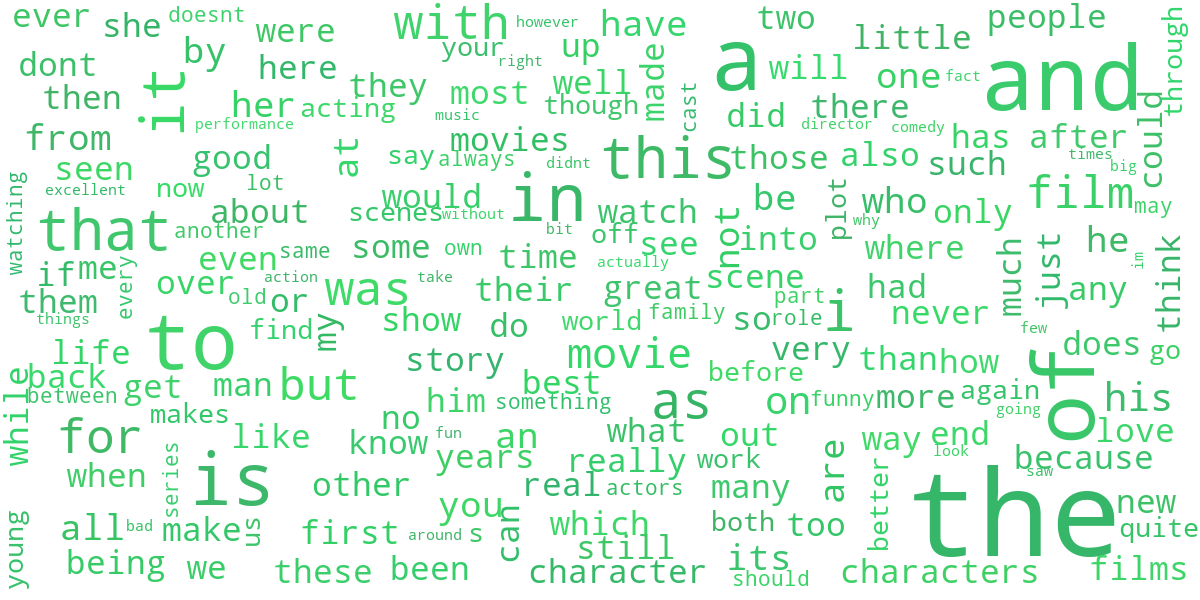
\includegraphics[width=0.44\textwidth]{../Q1/plots/wc_pos.png} & 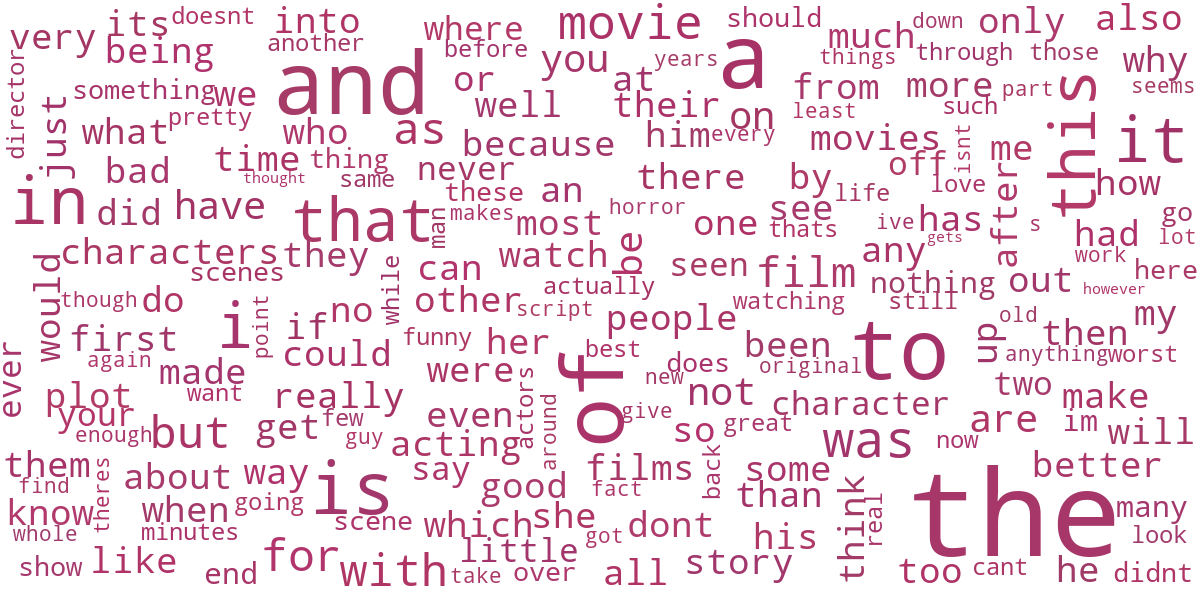
\includegraphics[width=0.44\textwidth]{../Q1/plots/wc_neg.png} \\
            Positive reviews & Negative reviews
        \end{tabular}
    \end{center}
    
    \item With Random Guessing, we'd obtain a test set accuracy of approximately 50\%. By simply predicting each sample as positive, this would jump to 66.6\%, as the number of positive reviews in the test set is twice the number of negative reviews.

    Our Algorithm gives a 30\% increase in accuracy over random guessing and a 14\% increase in accuracy over simply predicting each review as positive.

    \item The confusion matrices are as follows:

    \begin{center}
    \begin{tabular}{c c c}
        NaiveBayes & Random & AllPositive \\
        \begin{tabular}{r|c|c|}
            & AP & AN \\
            \hline
            PP & 7501 & 604 \\
            \hline
            PN & 2499 & 4396 \\
            \hline
        \end{tabular} & 
        \begin{tabular}{r|c|c|}
            & AP & AN \\
            \hline
            PP & 5000 & 2500 \\
            \hline
            PN & 5000 & 2500 \\
            \hline
        \end{tabular} &
        \begin{tabular}{r|c|c|}
            & AP & AN \\
            \hline
            PP & 10000 & 5000 \\
            \hline
            PN & 0 & 0 \\
            \hline
        \end{tabular} 
    \end{tabular}
    \end{center}

    TODO part 2 of this: wdym "highest value of diagonal entry"?

    The pattern is that the column sums for the actuals always add up to the number of examples of that category in the training set. This is because the actual column measures the number of actual examples in the dataset, and across all predictions, would sum to the total number of that category in the dataset.

    \item Removing stopwords and stemming gives us an accuracy of \textbf{80.4\%}, with 7678/10000 positive reviews and 4388/5000 negative reviews correctly classified.

    \begin{center}
        \begin{tabular}{c c}
            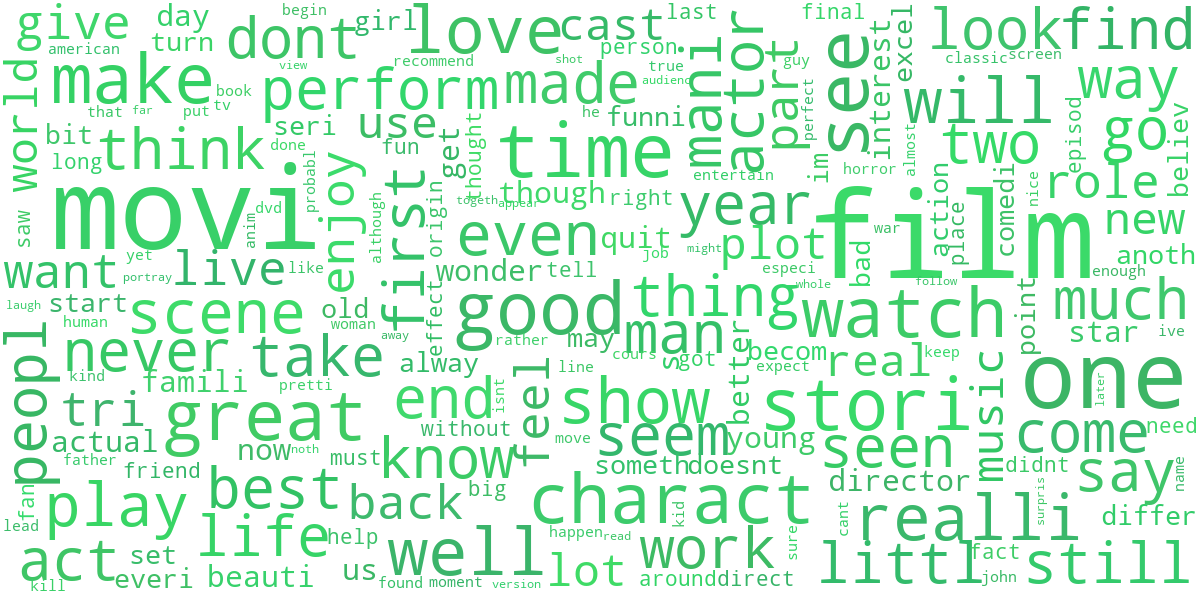
\includegraphics[width=0.44\textwidth]{../Q1/Qd/wc_pos.png} & 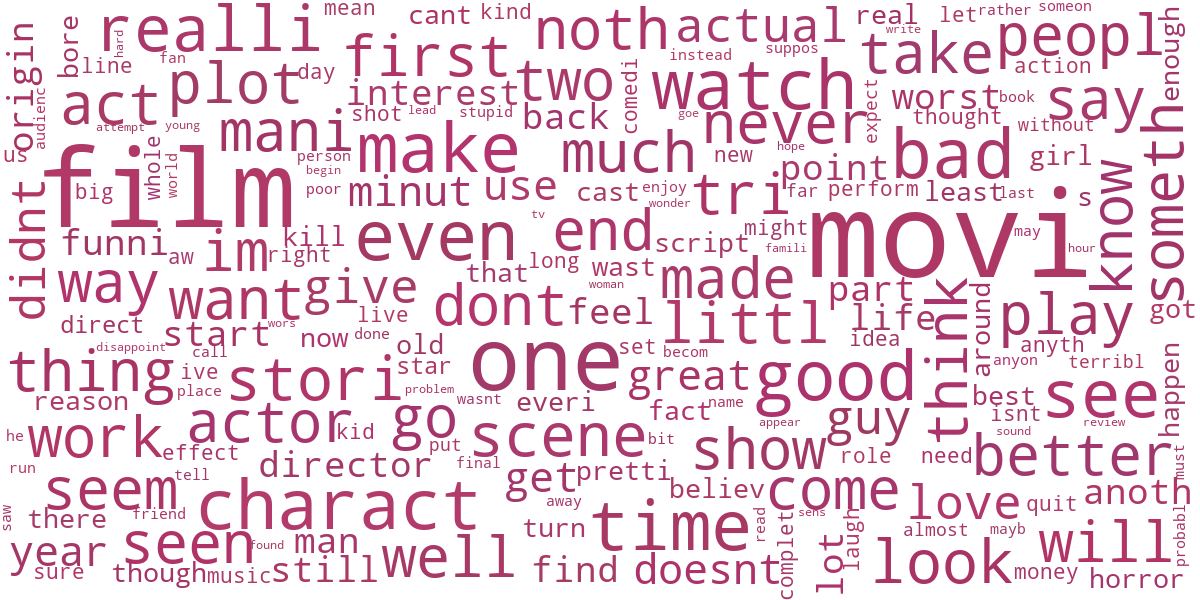
\includegraphics[width=0.44\textwidth]{../Q1/Qd/wc_neg.png} \\
            Positive reviews & Negative reviews
        \end{tabular}
    \end{center}

    The word clouds show the frequency of the various word stems rather than the frequency of the words themselves.

\item Using Bigrams (in addition to removing stopwords and stemming) gives us an accuracy of \textbf{84.4 \%}, with 8209/10000 positive reviews and 4447/5000 negative reviews correctly classified.

    For the additional feature, we use Trigrams. Using trigrams, in addition to bigrams and removing stopwords + stemming gives us an accuracy of \textbf{85.2 \%}, with 8352/10000 positive reviews and 4423/5000 negative reviews correctly classified.

    The additional sets of features do help us improve our accuracy (explain why)

\item The best-performing (most accurate) model is the Trigram model, which has a precision of 8352/(8352+577) = 0.935, a recall of 8352/(8352+1648) = 0.835 and an F1 score of $2(0.935 \times 0.835)/(0.935+0.835) = 0.882$

    The F1 score is a better metric for this dataset, as there are twice as many positive movie reviews in the test dataset compared to negative reviews. In this case, we can see significant accuracy gains by simply declaring everything as positive instead of proceeding class by class. The F1 score helps to prevent this from happening, and gives a more realistic representation of how accurate our model is, across both classes irrespective of how many samples there are in each class.

\end{enumerate}

\clearpage

\section{Binary SVM}

\section{Multiclass SVM}

\end{document}
